\documentclass{article}
\usepackage{neurips_2023}

\usepackage[utf8]{inputenc} % allow utf-8 input
\usepackage[T1]{fontenc}    % use 8-bit T1 fonts
\usepackage{hyperref}       % hyperlinks
\usepackage{url}            % simple URL typesetting
\usepackage{booktabs}       % professional-quality tables
\usepackage{amsfonts}       % blackboard math symbols
\usepackage{nicefrac}       % compact symbols for 1/2, etc.
\usepackage{microtype}      % microtypography
\usepackage{xcolor}         % colors
\usepackage{graphicx}       % images & graphics

\title{Man, I Just Love Writing Research Papers}
\author{%
  Jacob Badolato \\
  University of Texas at Austin \\
  \texttt{email@example.com} \\
  \And
  Andrew McGehee \\
  University of Texas at Austin \\
  \texttt{email@example.com} \\
}

\begin{document}

\maketitle

\begin{abstract}
  Many state of the art models perform very well across a broad spectrum of NLP tasks, however, detecting complex language patterns is still difficult. Though this can be achieved through many different routes, we propose that the simplest may be to re-train a well performing model on a small set of difficult examples. Analysis on the ELECTRA-SMALL model, trained on the SNLI dataset shows that re-training the model on a small set of challenging examples can increase the accuracy on detecting sarcasm by well over 50\%. This is a substantial increase, and the original model’s accuracy only dropped by a mere 1%. We show that through providing better training examples, a model can significantly improve its accuracy on various complex language patterns. 
\end{abstract}

\section{Introduction}
In the evolving field of NLP, the performance of state-of-the-art models is continually being pushed to new heights. 
These models excel across a broad spectrum of tasks, yet they often stumble when presented with complex language patterns. 
This paper explores a simple approach to enhancing model performance in such scenarios. We focus on the ELECTRA-SMALL model, 
a prominent player in the NLP domain.

Despite its capabilities, the ELECTRA-SMALL model, like many in its class, struggles with intricate linguistic constructs such as sarcasm, 
informal language, and figures of speech. These elements of language, often context-dependent and counter-intuitive, present a significant hurdle 
for these systems. Our study proposes a solution to this, rooted in targeted retraining.

We hypothesize that retraining a well-performing model on a carefully curated set of difficult examples can dramatically improve its ability 
to decipher these complex language patterns. To test this, we conducted an in-depth analysis of the ELECTRA-SMALL model, initially trained 
on the SNLI dataset. Our methodology involved appending to this training data with a selection of challenging examples, honing in on areas 
where the model historically underperformed.

This paper presents our findings, which indicate a substantial improvement in the model's ability to recognize and interpret sarcasm, rising by 
over 50\% in accuracy. Notably, this enhancement did not significantly detract from the model's overall performance on standard tasks, with 
only a minimal drop in accuracy observed. We will discuss the implications of these results, shedding light on the potential for hand-annotating
targeted examples to better handle the nuances of human language.

\section{Background}

\subsection{Challenges in Natural Language Processing}
These days, state-of-the-art NLP models perform quite well among a broad range of tasks. However, there remains significant progress
to be had when it comes to detecting complex language patterns such as, but not limited to, informal speech, sarcasm, and figures of speech. The title
of this paper alone shows that. 
\subsection{The ELECTRA-SMALL Model}
The ELECTRA-SMALL model was chosen because it is quicker to train than other models, and has less parameters, even though it is a robust
model that outperforms many larger models. However, it's performance drops off significantly when given certain nuances in the English language.
\subsection{Advancements in Model Retraining}
Recent advancements in the field of NLP have shown that having a pristine training dataset is one of the most fundamental aspects
of model performance. This approach promises to deepen the understanding we have of the relationship between good training data and 
understanding complex language structures.
\subsection{The Role of the SNLI Dataset}
The Stanford Natural Language Inference (SNLI) dataset has been pivotal in training numerous NLP models, including ELECTRA-SMALL. 
While it provides a broad spectrum of linguistic examples, its coverage of intricate language patterns is \href{https://nlp.stanford.edu/blog/the-stanford-nli-corpus-revisited/}{limited}. This limitation has 
prompted the exploration of supplemental training to bridge these gaps.



\section{Examples of Errors}
\subsection{Informal Speech}
\begin{itemize}
\item Premise: He doesn’t hardly speak to anyone.
\item Hypothesis: He is very outgoing.
\item Gold label: 2
\item Actual: 0
\end{itemize}

\subsection{Sarcasm}
\begin{itemize}
\item Premise: What a pleasant surprise, another bill in the mail.
\item Hypothesis: I do not enjoy paying my bills.
\item Gold label: 2
\item Actual: 0
\end{itemize}
  
\subsection{Figures of Speech}
\begin{itemize}
\item Premise: Come on, spill the beans about the party plans!
\item Hypothesis: Someone wants them to spill the beans about the party plans.
\item Gold label: 0
\item Actual: 1
\end{itemize}

\newpage
\section{Discussion on Retraining the Model}
The general class of mistakes that we tested fell into three categories. These categories consist of examples in which there exists a negation of sorts 
(especially double negation), those which use sarcasm, and those that use figures of speech. The above categories are difficult for the model to interpret because
they each have unorthodox or non-literal usages. These findings suggest that the model struggles the most with context-dependent and counter-intuitive examples. We 
believe that provided more context, or with more sophisticated linguistic analysis, the model would perform significantly better. Figure 1 shows the different error
rates for the three classes.

\begin{figure}[!h]
  \centering
  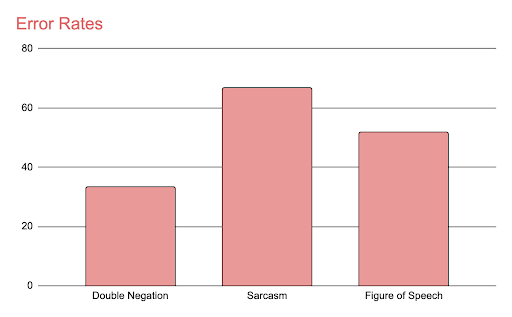
\includegraphics[width=0.5\textwidth]{images/error_rates.png}
  \caption{error rates}
  \label{fig:a}
\end{figure}

Using a confusion matrix, we can more deeply understand what kind of misclassifications the model is making. We can see from the data that the model has a very 
difficult time classifying examples where the true label is 2, as compared to those with a true label of 0 or 1. This is expected, because many of our examples 
are supposed to make the model think it is entailment, when really it is a contradiction. Figure 2 illustrates this below. Figure 3 shows the confusion 
matrix for the SNLI dataset, which when evaluated on the checkpoint we chose, has an accuracy of 85.8\%. 

\begin{figure}[!h]
  \centering
  \begin{minipage}{0.46\textwidth}
    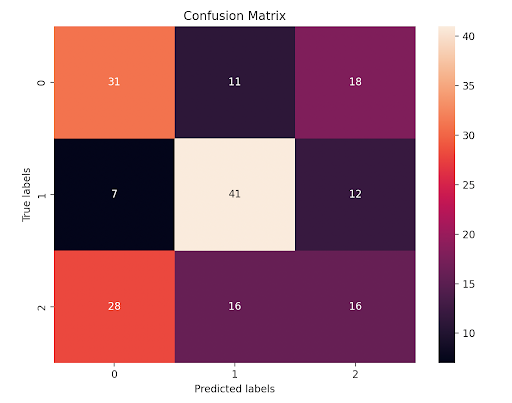
\includegraphics[width=\linewidth]{images/confusion_trained_tricky.png}
    \caption{tricky examples (pre-tuning)}
    \label{fig:b}
  \end{minipage}
  \hfill
  \begin{minipage}{0.48\textwidth}
    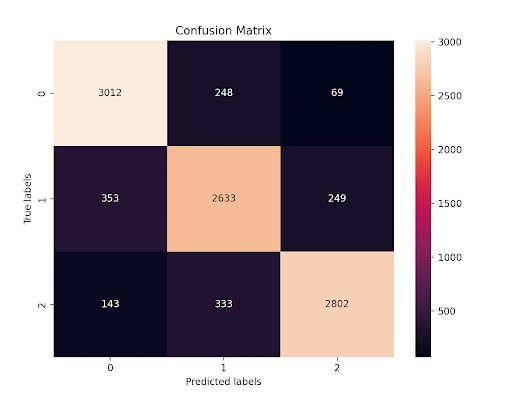
\includegraphics[width=\linewidth]{images/confusion_trained_snli.png}
    \caption{snli dataset (pre-tuning)}
    \label{fig:c}
  \end{minipage}
\end{figure}

As one can see, the model performs significantly worse on our “tricky examples” dataset than on the original SNLI training dataset. This is to be expected, and 
now we will go about fixing it. 

\section{The Fix is In}
To fix our project, we ended up retraining the model with our hand-annotated examples. We used 60 different examples for each category (double negation, figure of 
speech, and sarcasm) with each example containing three sentences. One sentence was entailment, one was neutral, and the last was a contradiction. This gave us a 
total of 180 sentences in whole. After retraining the data on the SNLI dataset with our examples included, our model accuracy jumped to 75\% on the “tricky examples”, 
up from 49\%. The respective confusion matrices are shown below in figures 4 (tuned model) and 5 (original model).

\begin{figure}[!h]
  \centering
  \begin{minipage}{0.47\textwidth}
    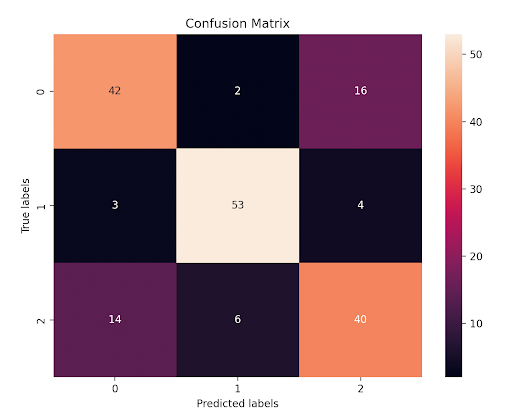
\includegraphics[width=\linewidth]{images/confusion_tuned_tricky.png}
    \caption{tuned on tricky examples}
    \label{fig:d}
  \end{minipage}
  \hfill
  \begin{minipage}{0.47\textwidth}
    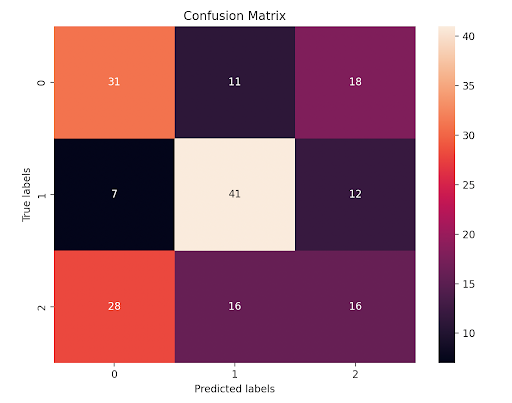
\includegraphics[width=\linewidth]{images/confusion_trained_tricky.png}
    \caption{trained on tricky examples}
    \label{fig:e}
  \end{minipage}
\end{figure}

When evaluating the same metrics on the SNLI dataset, however, we got very different results. We found that our accuracy on the SNLI dataset actually decreased to 
84.6\% compared to 85.8\% originally. This drop in accuracy can be explained by something known as “catastrophic forgetting”, and is expected behavior since we 
retrained the model with new examples that were significantly different from the original. Catastrophic forgetting is a byproduct of sequential learning, and occurs 
when a model is trained for task A, and then retrained for task B. This will cause the model to be better at task B, but perform worse on task A. This is because the 
weights, which were optimized for task A, get updated for task B, potentially losing the information relevant to task A. It should be noted, however, that the model 
reduced misclassification in the neutral sentiment class, and did not change accuracy in the entailment category. The corresponding confusion matrices are shown below 
in figures 5 and 6. 

\begin{figure}[!h]
  \centering
  \begin{minipage}{0.44\textwidth}
    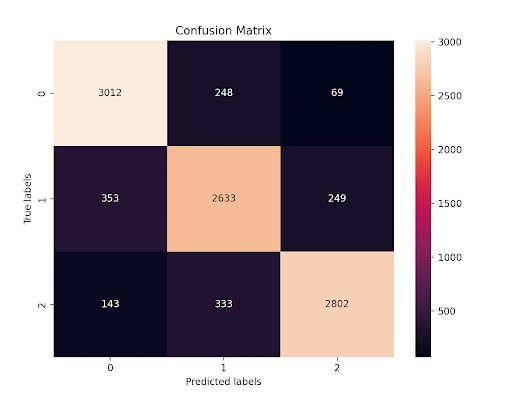
\includegraphics[width=\linewidth]{images/confusion_trained_snli.png}
    \caption{trained on snli dataset}
    \label{fig:f}
  \end{minipage}
  \hfill
  \begin{minipage}{0.44\textwidth}
    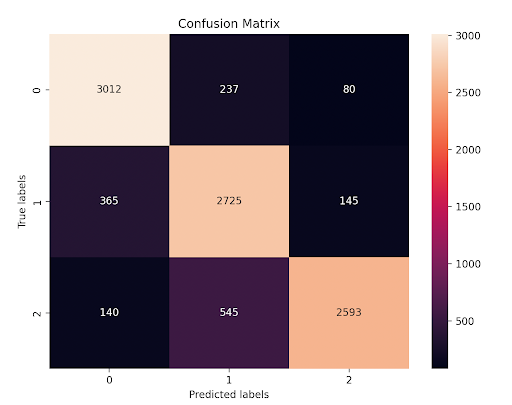
\includegraphics[width=\linewidth]{images/confusion_tuned_snli.png}
    \caption{SNLI tuned with tricky examples}
    \label{fig:g}
  \end{minipage}
\end{figure}

\newpage
Also notable in our findings are the accuracy, precision, recall, and f1 scores. Both models had a tight cluster of the aforementioned metrics, with each metric being 
within 1\% of each other (figure 8). 

\begin{figure}[!h]
  \centering
  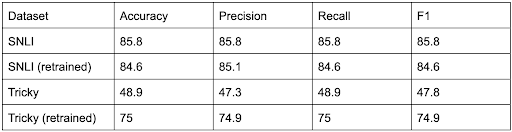
\includegraphics[width=\linewidth]{images/metrics_nlp_final_project.png}
  \caption{metrics}
  \label{fig:h}
\end{figure}

As noted in figure 8, and supported by the confusion matrices, the model is relatively balanced. This is important to note because it shows that the changes in our performance 
on comples language structes was not due to an inconsistent model, or inconsistent learning. 

\section{Conclusion}

To conclude, this paper introduces a method that effectively enhances the performance of NLP models in processing complex language structures, while  
preserving their overall performance. We demonstrate that retraining the model with a thoughtfully selected set of hand-annotated examples, specifically designed to challenge 
the model, can lead to significant improvements. However, it's crucial to use caution during the retraining process to prevent catastrophic forgetting. This involves a careful 
consideration of the number and nature of examples used, ensuring they aid the model's learning without overwhelming the existing weights. This approach underscores 
the potential of targeted retraining as a powerful tool in refining state-of-the-art models.

\end{document}
